\documentclass[11pt,a4paper]{article}
\usepackage[utf8]{inputenc}
\usepackage[english]{babel}
\usepackage[T1]{fontenc}
\usepackage{amsmath}
\usepackage{amsfonts}
\usepackage{amssymb}
\usepackage{graphicx}
\usepackage{epstopdf}
\setlength{\parindent}{4em} 
\author{Jakub Drápela}
\usepackage{fancyhdr}
\usepackage{siunitx}
\graphicspath{{./figures/}}
\usepackage{wrapfig}

%\fontfamily{phs}
%\selectfont
\usepackage[backend=bibtex,style=numeric]{biblatex}
\usepackage{filecontents}  % create "citations.bib" on-the-fly

\begin{document}
\pagestyle{empty}

%%nastaveni pisma  
%\fontfamily{phv}
%\selectfont

	\begin{center}

\large

České vysoké učení technické v Praze

\medskip

Elektrotechnická fakulta
\vfill
\vfill
{\LARGE\bfseries Skupiny svazků}


\vspace{15mm}

\vfill
\vfill
\vfill

{\LARGE\bfseries CMP}

\vfill

\begin{tabular}{rl}

Autor: & Jakub Drápela \\
\noalign{\vspace{2mm}}
Studijní obor: & Kybernetika a robotika \\
\noalign{\vspace{2mm}}
Datum vypracování: & \today\\
\end{tabular}

\end{center}

\newpage
\pagestyle{plain}     % zapne obyčejné číslování
\setcounter{page}{1}  % nastaví čítač stránek znovu od jedné  
\subsection{Předchozí verze z bakalářské práce}
\label{sec:hdr_image}
\indent	Použitím HDR (High Dynamic Range) snímku zajistíme pokrytí velkého dynamického rozsahu. Jedním z možností rekonstrukce HDR obrázku je složení obrázku ze snímků s různými expozicemi. U pořizování snímku volíme takové expozice, abychom jednotlivými snímky pokryli celý dynamický rozsah jasu. Dobu expozice postupně snižujeme dokud nejsou hodnoty jasu všech pixelů bez saturace.   \\
\indent	Laserový svazek si představujeme jako tok fotonů o určité vlnové délce. Při rekonstrukci HDR obrázku počítáme počet fotonů dopadených na snímací čip za jednotku času (intenzita $ I $). Ze snímku vybereme nesaturované pixely a jejich intenzitu vydělíme časem expozice. Celkovou intenzitu pixelu určíme jako vážený průměr všech expozic bez saturace. Vyjádřeno vztahem:  
\begin{eqnarray}
		I = \frac{\sum\limits_{i = i_{nesat}}^nj_i}{\sum\limits_{i =i_{nesat}}^nt_i}\,.
		\quad\quad\quad
		\begin{array}{ccc}
   		i_{nesat}&-&\mbox{první nesaturovaná expozice} \\
   		j&-&\mbox{jas pixelu} \\
   		t&-&\mbox{čas expozice} 
 		\end{array}
		\label{eq:HDR1}
\end{eqnarray}

\subsection{Změna v nové verzi}

Algoritmus pro skládání obrázku byl změněn a nyní má následující tvar:

\begin{eqnarray}
		I = \frac{\sum\limits_{i = i_{nesat}}^n j_i\,\sqrt{t_i}}{\sum\limits_{i =i_{nesat}}^n t_i\,\sqrt{t_i}}\,.
		\quad\quad\quad
		\begin{array}{ccc}
   		i_{nesat}&-&\mbox{první nesaturovaná expozice} \\
   		j&-&\mbox{jas pixelu} \\
   		t&-&\mbox{čas expozice} 
 		\end{array}
		\label{eq:HDR2}
\end{eqnarray}

\subsection{Porovnání algoritmů}
Pro porovnání algoritmů \ref{eq:HDR1} a \ref{eq:HDR2} byl proveden nestranný odhad, pří kterém se posuzovala vydatnost (eficience obou algoritmů). K posouzení vydatnosti bylo použito 10 sérií snímků totožné scény se širokou škálou expozic. Na každou sérii snímků s různými expozicemi byl aplikován algoritmus \ref{eq:HDR1} resp. \ref{eq:HDR2} a vypočten HDR snímkem. Takto tedy vzniklo od každého algoritmu 10 různých HDR snímků. 

Posouzení vydatnosti spočívá v tom, že jako věrohodný odhad určí ten s menším rozptylem. Pro totožné pixely ve všech 10 snímcích byl vypočten rozptyl a rozptyl všech pixelů sečten. Výsledek je zaznamenán v tabulce \ref{tab: porovnani}.

\begin{table}[h!]


\begin{tabular}{c|c|c}

Výpočetní metoda		&	Rozptyl  			&	 Směrodatná odchylka/Pixel\\
\hline\hline
Rovnice \ref{eq:HDR1} 	&	$3.479\times10^7$	& $2.877$\\
\hline
Rovnice \ref{eq:HDR2}	&	$2.899\times10^7$	& $2.627$


\end{tabular}   
 
\caption{Výsledky porovnání dvou algoritmů pro výpočet HDR snímku.}
\label{tab: porovnani} 
\end{table}



\begin{table}
\centering
\begin{tabular}{|c|c|c|c|c|c|c|c|c|c|c|c|}

\hline
Combination &  &  &  &  &  &  &  &  &  &  & Separability \\
\hline
\textbf{23} & 10 & 60 & 61 & 62 & 70 & 90 & 30 & 63 & 71 & 80 & 0.815 \\
\hline
\textbf{21} & 10 & 60 & 61 & 62 & 70 & 71 & 30 & 63 & 80 & 90 & 0.800 \\
\hline
\textbf{49} & 30 & 60 & 61 & 62 & 70 & 71 & 10 & 63 & 80 & 90 & 0.790 \\
\hline
\textbf{40} & 10 & 61 & 62 & 63 & 70 & 80 & 30 & 60 & 71 & 90 & 0.789 \\
\hline
\textbf{18} & 10 & 60 & 61 & 62 & 63 & 71 & 30 & 70 & 80 & 90 & 0.779 \\
\hline
\textbf{29} & 10 & 60 & 61 & 63 & 70 & 90 & 30 & 62 & 71 & 80 & 0.779 \\
\hline
\textbf{35} & 10 & 60 & 62 & 63 & 70 & 90 & 30 & 61 & 71 & 80 & 0.779 \\
\hline
\textbf{27} & 10 & 60 & 61 & 63 & 70 & 71 & 30 & 62 & 80 & 90 & 0.769 \\
\hline
\textbf{33} & 10 & 60 & 62 & 63 & 70 & 71 & 30 & 61 & 80 & 90 & 0.769 \\
\hline
\textbf{42} & 10 & 61 & 62 & 63 & 71 & 80 & 30 & 60 & 70 & 90 & 0.765 \\
\hline
\textbf{16} & 10 & 30 & 61 & 62 & 63 & 90 & 60 & 70 & 71 & 80 & 0.762 \\
\hline
\textbf{57} & 30 & 60 & 61 & 63 & 70 & 90 & 10 & 62 & 71 & 80 & 0.760 \\
\hline
\textbf{63} & 30 & 60 & 62 & 63 & 70 & 90 & 10 & 61 & 71 & 80 & 0.760 \\
\hline
\textbf{13} & 10 & 30 & 61 & 62 & 63 & 70 & 60 & 71 & 80 & 90 & 0.755 \\
\hline
\textbf{44} & 10 & 61 & 62 & 63 & 80 & 90 & 30 & 60 & 70 & 71 & 0.754 \\
\hline
\textbf{4} & 10 & 30 & 60 & 61 & 62 & 90 & 63 & 70 & 71 & 80 & 0.754 \\
\hline
\textbf{50} & 30 & 60 & 61 & 62 & 70 & 80 & 10 & 63 & 71 & 90 & 0.751 \\
\hline
\textbf{51} & 30 & 60 & 61 & 62 & 70 & 90 & 10 & 63 & 71 & 80 & 0.751 \\
\hline
\textbf{58} & 30 & 60 & 61 & 63 & 71 & 80 & 10 & 62 & 70 & 90 & 0.750 \\
\hline
\textbf{64} & 30 & 60 & 62 & 63 & 71 & 80 & 10 & 61 & 70 & 90 & 0.750 \\
\hline
\textbf{31} & 10 & 60 & 61 & 63 & 71 & 90 & 30 & 62 & 70 & 80 & 0.750 \\
\hline
\textbf{37} & 10 & 60 & 62 & 63 & 71 & 90 & 30 & 61 & 70 & 80 & 0.750 \\
\hline
\textbf{22} & 10 & 60 & 61 & 62 & 70 & 80 & 30 & 63 & 71 & 90 & 0.748 \\
\hline
\textbf{30} & 10 & 60 & 61 & 63 & 71 & 80 & 30 & 62 & 70 & 90 & 0.748 \\
\hline
\textbf{36} & 10 & 60 & 62 & 63 & 71 & 80 & 30 & 61 & 70 & 90 & 0.748 \\
\hline
\textbf{41} & 10 & 61 & 62 & 63 & 70 & 90 & 30 & 60 & 71 & 80 & 0.748 \\
\hline
\textbf{45} & 30 & 60 & 61 & 62 & 63 & 70 & 10 & 71 & 80 & 90 & 0.746 \\
\hline
\textbf{54} & 30 & 60 & 61 & 62 & 80 & 90 & 10 & 63 & 70 & 71 & 0.746 \\
\hline
\textbf{6} & 10 & 30 & 60 & 61 & 63 & 71 & 62 & 70 & 80 & 90 & 0.745 \\
\hline
\textbf{10} & 10 & 30 & 60 & 62 & 63 & 71 & 61 & 70 & 80 & 90 & 0.745 \\
\hline
\textbf{28} & 10 & 60 & 61 & 63 & 70 & 80 & 30 & 62 & 71 & 90 & 0.745 \\
\hline
\textbf{34} & 10 & 60 & 62 & 63 & 70 & 80 & 30 & 61 & 71 & 90 & 0.745 \\
\hline
\textbf{56} & 30 & 60 & 61 & 63 & 70 & 80 & 10 & 62 & 71 & 90 & 0.744 \\
\hline
\textbf{62} & 30 & 60 & 62 & 63 & 70 & 80 & 10 & 61 & 71 & 90 & 0.744 \\
\hline
\textbf{14} & 10 & 30 & 61 & 62 & 63 & 71 & 60 & 70 & 80 & 90 & 0.744 \\
\hline
\textbf{53} & 30 & 60 & 61 & 62 & 71 & 90 & 10 & 63 & 70 & 80 & 0.743 \\
\hline
\textbf{48} & 30 & 60 & 61 & 62 & 63 & 90 & 10 & 70 & 71 & 80 & 0.743 \\
\hline
\textbf{52} & 30 & 60 & 61 & 62 & 71 & 80 & 10 & 63 & 70 & 90 & 0.743 \\
\hline
\textbf{8} & 10 & 30 & 60 & 61 & 63 & 90 & 62 & 70 & 71 & 80 & 0.742 \\
\hline
\textbf{12} & 10 & 30 & 60 & 62 & 63 & 90 & 61 & 70 & 71 & 80 & 0.742 \\
\hline
\textbf{25} & 10 & 60 & 61 & 62 & 71 & 90 & 30 & 63 & 70 & 80 & 0.742 \\
\hline
\end{tabular}
\caption{Graph of mean separability on used combination of rays}
\label{table:MeanSeperability}
\end{table}

\newpage
\begin{table}
\centering
\begin{tabular}{|c|c|c|c|c|c|c|c|c|c|c|c|}

\hline
Combination &  &  &  &  &  &  &  &  &  &  & Separability \\
\hline
\textbf{32} & 10 & 60 & 61 & 63 & 80 & 90 & 30 & 62 & 70 & 71 & 0.740 \\
\hline
\textbf{38} & 10 & 60 & 62 & 63 & 80 & 90 & 30 & 61 & 70 & 71 & 0.740 \\
\hline
\textbf{24} & 10 & 60 & 61 & 62 & 71 & 80 & 30 & 63 & 70 & 90 & 0.738 \\
\hline
\textbf{5} & 10 & 30 & 60 & 61 & 63 & 70 & 62 & 71 & 80 & 90 & 0.738 \\
\hline
\textbf{9} & 10 & 30 & 60 & 62 & 63 & 70 & 61 & 71 & 80 & 90 & 0.738 \\
\hline
\textbf{3} & 10 & 30 & 60 & 61 & 62 & 80 & 63 & 70 & 71 & 90 & 0.736 \\
\hline
\textbf{43} & 10 & 61 & 62 & 63 & 71 & 90 & 30 & 60 & 70 & 80 & 0.733 \\
\hline
\textbf{17} & 10 & 60 & 61 & 62 & 63 & 70 & 30 & 71 & 80 & 90 & 0.730 \\
\hline
\textbf{39} & 10 & 61 & 62 & 63 & 70 & 71 & 30 & 60 & 80 & 90 & 0.729 \\
\hline
\textbf{59} & 30 & 60 & 61 & 63 & 71 & 90 & 10 & 62 & 70 & 80 & 0.729 \\
\hline
\textbf{65} & 30 & 60 & 62 & 63 & 71 & 90 & 10 & 61 & 70 & 80 & 0.729 \\
\hline
\textbf{1} & 10 & 30 & 60 & 61 & 62 & 70 & 63 & 71 & 80 & 90 & 0.727 \\
\hline
\textbf{55} & 30 & 60 & 61 & 63 & 70 & 71 & 10 & 62 & 80 & 90 & 0.726 \\
\hline
\textbf{61} & 30 & 60 & 62 & 63 & 70 & 71 & 10 & 61 & 80 & 90 & 0.726 \\
\hline
\textbf{2} & 10 & 30 & 60 & 61 & 62 & 71 & 63 & 70 & 80 & 90 & 0.722 \\
\hline
\textbf{15} & 10 & 30 & 61 & 62 & 63 & 80 & 60 & 70 & 71 & 90 & 0.718 \\
\hline
\textbf{60} & 30 & 60 & 61 & 63 & 80 & 90 & 10 & 62 & 70 & 71 & 0.714 \\
\hline
\textbf{66} & 30 & 60 & 62 & 63 & 80 & 90 & 10 & 61 & 70 & 71 & 0.714 \\
\hline
\textbf{20} & 10 & 60 & 61 & 62 & 63 & 90 & 30 & 70 & 71 & 80 & 0.710 \\
\hline
\textbf{7} & 10 & 30 & 60 & 61 & 63 & 80 & 62 & 70 & 71 & 90 & 0.709 \\
\hline
\textbf{11} & 10 & 30 & 60 & 62 & 63 & 80 & 61 & 70 & 71 & 90 & 0.709 \\
\hline
\textbf{26} & 10 & 60 & 61 & 62 & 80 & 90 & 30 & 63 & 70 & 71 & 0.707 \\
\hline
\textbf{46} & 30 & 60 & 61 & 62 & 63 & 71 & 10 & 70 & 80 & 90 & 0.698 \\
\hline
\textbf{47} & 30 & 60 & 61 & 62 & 63 & 80 & 10 & 70 & 71 & 90 & 0.651 \\
\hline
\textbf{19} & 10 & 60 & 61 & 62 & 63 & 80 & 30 & 70 & 71 & 90 & 0.626 \\
\hline
\end{tabular}
\caption{Table of mean separability on used combination of rays.}
\label{table:MeanSeperability}
\end{table}

\newpage

\begin{figure}[htp]
\centering
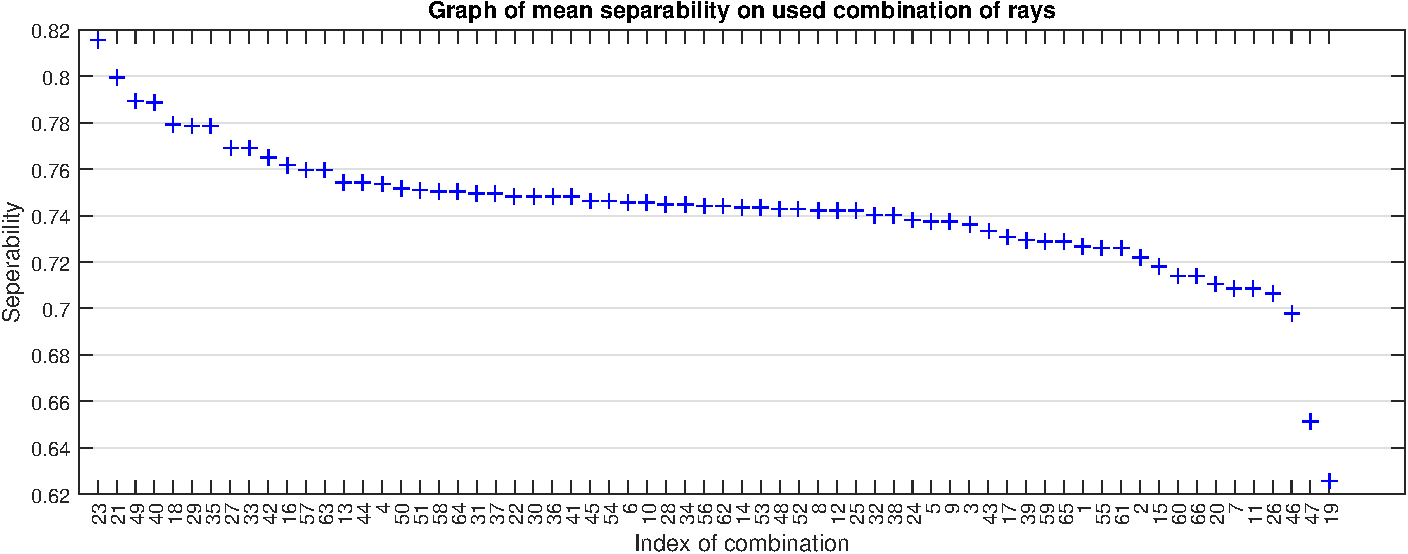
\includegraphics[width=14cm]{MeanSeperability.pdf}
\caption{Graph of mean separability on used combination of rays.}
\end{figure}


\begin{table} [htp]
\centering
\begin{tabular}{|c|c|c|c|c|c|c|c|c|c|c|}
\hline 
 Ray group & 10 & 30 & 60 & 61 & 62 & 63 & 80  & 70 & 71 & 90\\
\hline
Separability & 0.617 & 0.698 & 0.706 & - & - & 0.696 & 0.707 & 0.697 & 0.617 & 0.654 \\
\hline
Set size &3825 & 5626 & 2703 & - & - & 3490 & 8195 & 8350 & 8356 & 8459 \\
\hline
\end{tabular}
\caption{Table of separability for each rays groupes.}
\label{table:GroupSeperability}
\end{table}


\clearpage
\nocite{*}
\printbibliography 

\end{document}
